\section{Spatio-Temporal Data Visualization}\label{sec:spatio-temporal-data-visualization}

In the previous sections, we briefly mentioned temporal and geospatial data visualizations which only take into
consideration time and space, respectively, but now we will look into data that relates to both space and time and some
ways of representing them.

Since we are talking about space, we are considering the geographical position of an object at a specific time.
The object is likely to move around different places at different times, thus allowing us to use the gathered
information and show it on a graph or map, in some two-dimensional or three-dimensional space. Spatio-temporal data increased massively with
technological development, especially the usage of mobile phones, Internet-based map services, GPS devices, weather
services, and digital Earth~\citep{han2022data}. This allowed people to search for innovative data representations
which would try to combine and show this information in the most useful and possible way. In earth sciences, where
patterns of temporal change are examined, such as global warming, population growth, or the spread of diseases,
spatio-temporal data is widely used~\citep{nollenburg2007geographic}.

According to the temporal variations over time, Andrienko et al.~\citep{andrienko2003exploratory} categorized
spatio-temporal data as follows:
\begin{enumerate}
    \item Existential changes, i.e., appearance and disappearance attributes.
    \item Changes of spatial properties such as location, shape, size, orientation, etc.
    \item Changes of thematic properties, i.e., qualitative changes and changes of numeric characteristics.
\end{enumerate}

In this research, we are interested in the second one -- changes in spatial properties over time, as the location of the
artist will be the main component of our visualization, as well as the third one -- representing qualitative and quantitative changes of aspects
of artists' lives.

Kjellin et al.~\citep{kjellin2008evaluating} state that there are three main spatio-temporal visualization types:
\begin{enumerate}
    \item 2D maps -- in addition to maps showing spatial data, time is often shown by specifically noting time stamps.
    \item Animations -- a technique used widely in geovisualization whose usual primary goal is not to show the movement of an object but to visualize other changing phenomena.
    \item Space-time cubes -- time dimension is orthogonal to the map on the surface making these cubes 3D visualization techniques.
\end{enumerate}

Considering two-dimensional space, a great example of spatio-temporal data visualization would be a chart by
Andrienko et al.~\citep{andrienko2005visual}, which shows the burglary rate distribution in the USA from 1960 to 2000.

\begin{figure}[hbt!]
    \begin{center}
        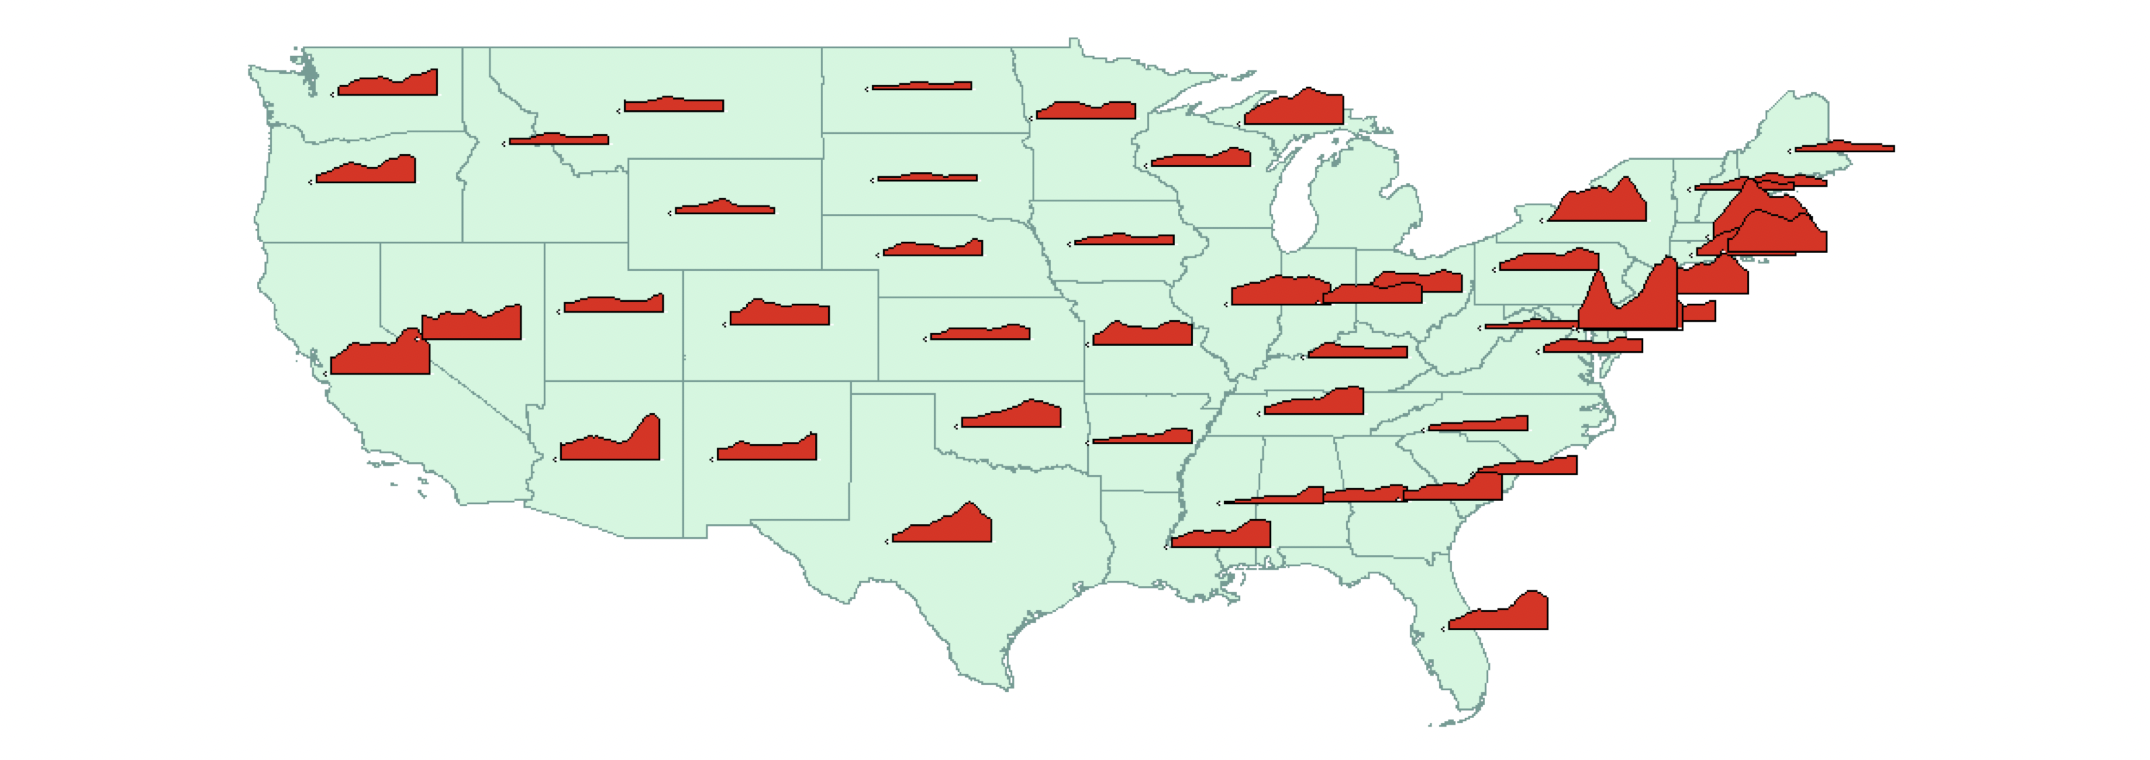
\includegraphics[width=0.9\textwidth]{graphics/2-literature-review/7}
    \end{center}
    \caption{A cartographic representation of the spatial distribution of burglary rates in the USA}
    \label{fig:figure2.7}
\end{figure}

Each state has its time graph to show the local behavior based on the location. The coordinate plot of the time
graph was neglected and the area between the timeframe was filled with color for better distinction on the map. This
map not only shows the local information for each state, but it is possible to notice multiple clusters across them as well.
In some states the burglary rate was always low, in others was always high, etc. Some states had variations in rates,
so this may lead to a conclusion that perhaps major changes in the law or system were adopted to prevent burglary at that time/year.
These kinds of observations can give us insightful information about common patterns of behaviors in certain states.

Switching to 3D visualizations, we talk about the previously mentioned space-time cubes. Since this type of representation
has great potential to be considered as a basis worth implementing in this research, we will dedicate a separate section
to explore it in detail.
